% LaTeX source for ``การเรียนรู้ของเครื่องสำหรับเคมีควอนตัม (Machine Learning for Quantum Chemistry)''
% Copyright (c) 2022 รังสิมันต์ เกษแก้ว (Rangsiman Ketkaew).

% License: Creative Commons Attribution-NonCommercial-NoDerivatives 4.0 International (CC BY-NC-ND 4.0)
% https://creativecommons.org/licenses/by-nc-nd/4.0/

{
\thispagestyle{empty}

\begin{center}
    \LARGE\textbf{ประวัติผู้เขียน}
\end{center}

\begin{minipage}[t][8cm][t]{\textwidth}
    \begin{wrapfigure}{l}{0.4\textwidth}
        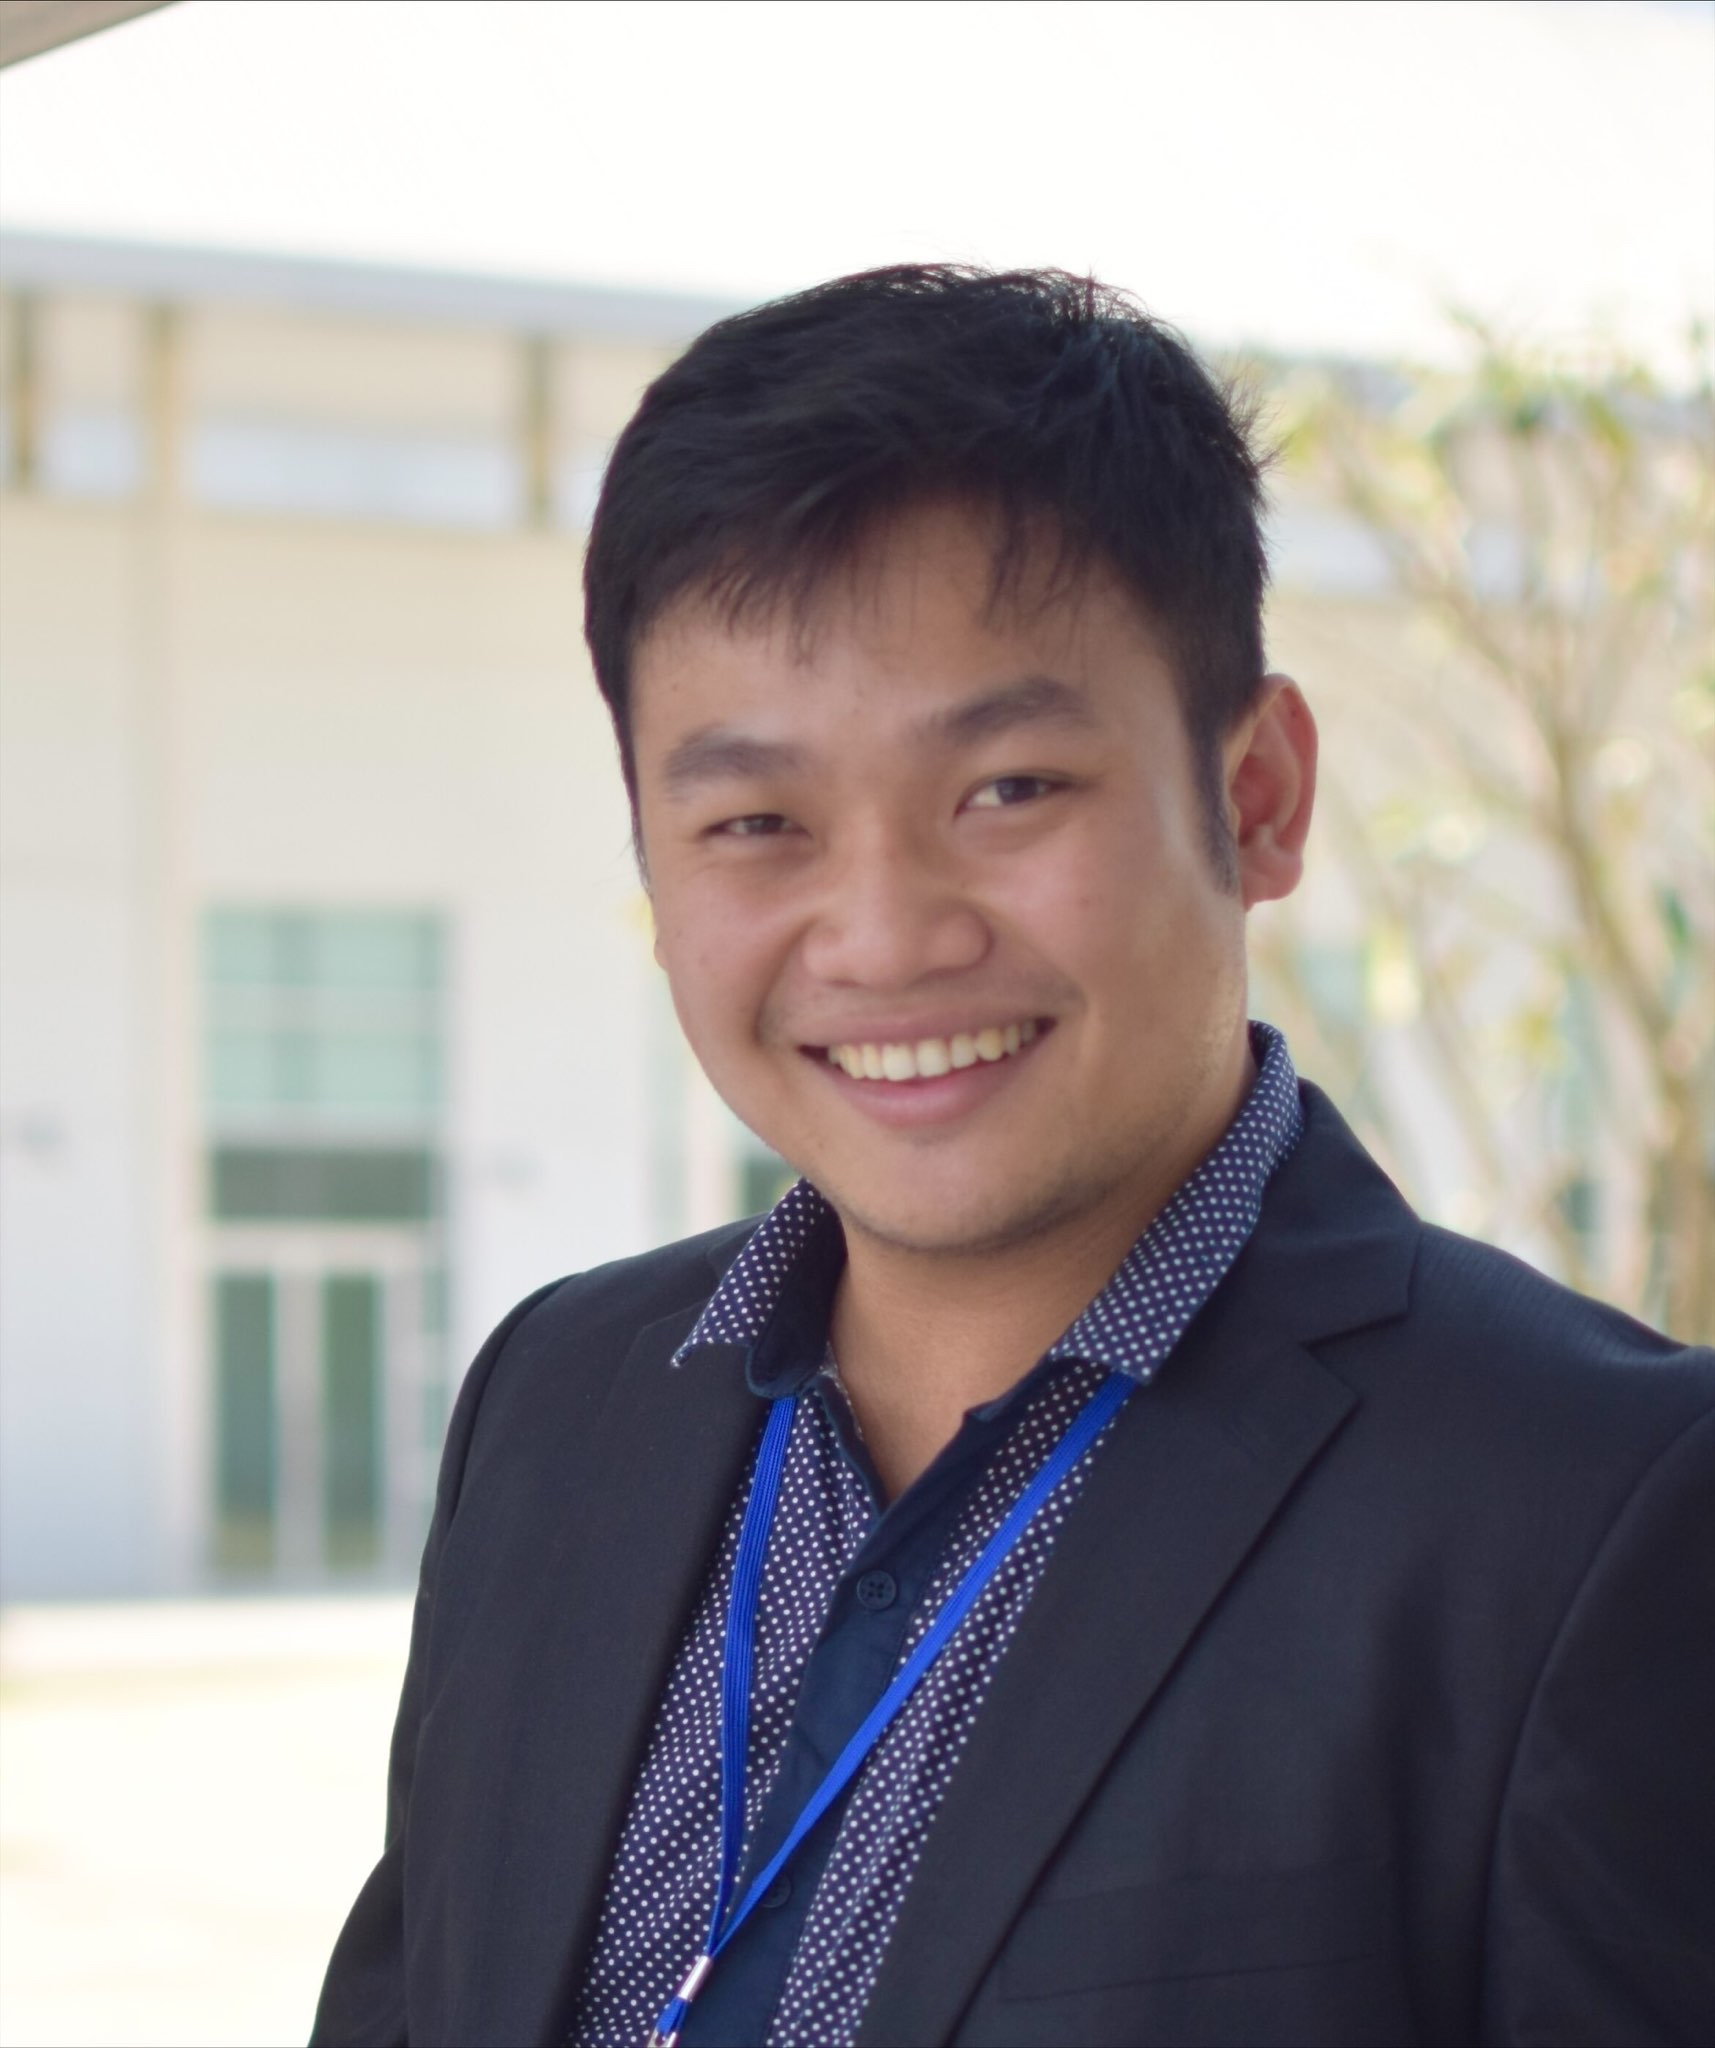
\includegraphics[width=0.85\linewidth]{fig/RK-profile.jpg}
    \end{wrapfigure}
    \leavevmode
    \\
    \hspace*{1em} รังสิมันต์ เกษแก้ว สำเร็จการศึกษาปริญญาตรี (พ.ศ. 2559) และปริญญาโท (พ.ศ. 2562) สาขาเคมี จากภาควิชาเคมี 
    คณะวิทยาศาสตร์และเทคโนโลยี มหาวิทยาลัยธรรมศาสตร์ ศูนย์รังสิต ปัจจุบันกำลังศึกษาปริญญาเอกสาขาเคมีทฤษฎีที่ภาควิชาเคมี 
    มหาวิทยาลัยแห่งซูริค ประเทศสวิตเซอร์แลนด์ หัวข้องานวิจัยที่สนใจ ได้แก่ เคมีควอนตัม เมตาไดนามิกส์ การถ่ายโอนอิเล็กตรอน ปัญญาประดิษฐ์ 
    และการพัฒนาซอฟต์แวร์ด้านเคมีเชิงคำนวณ
\end{minipage}

\leavevmode
\vspace{-3em}

\noindent ประสบการณ์การทำงาน
\vspace{-1em}
\begin{flushleft}
\begin{table}[H]
    \resizebox{\textwidth}{!}{%
    \begin{tabular}{ll}
        $\bullet$ พ.ศ. 2562-2563 &ที่ปรึกษาบริษัท New Equilibrium Biosciences, Boston, MA \\
        $\bullet$ พ.ศ. 2564 &ที่ปรึกษาบริษัท ติ๊งกิ้ง แมชชีนส์ จำกัด (Thinking Machines) \\
        $\bullet$ พ.ศ. 2564 &คณะกรรมการจัดการแข่งขันปัญญาประดิษฐ์สําหรับเคมีแห่งประเทศไทย \\
        $\bullet$ พ.ศ. 2564 &คณะกรรมการจัดงาน PyCon Thailand และ PyCon APAC 2021 \\
        $\bullet$ พ.ศ. 2565 &นักเขียนบทความบริษัท คลาวด์ เอชเอ็ม จำกัด (Cloud HM)
    \end{tabular}
    }
\end{table}
\end{flushleft}

\vspace{-2em}

\noindent ผู้ก่อตั้งเพจและกลุ่ม Facebook 
\vspace{-1em}
\begin{flushleft}
\begin{table}[H]
    \resizebox{0.53\textwidth}{!}{%
    \begin{tabular}{l}
        $\bullet$ วิทย์ตามิน \\
        $\bullet$ Machine Learning in Chemistry Thailand \\
        $\bullet$ CompChem Thailand \\
        $\bullet$ Thai Computational Science Students
    \end{tabular}
    }
\end{table}
\end{flushleft}

\vspace{-1em}

\noindent ดูบทความอื่น ๆ ของผู้เขียนได้ที่ \url{https://rangsimanketkaew.github.io}

\vfill
}
